%%%%%%%%%%%%%%%%%%%%%%%%%%%%%%%%%%%%%%%%%%%%%%%%%%%%%%%%%%%%%%%%%%%%%%%%%%%
%%
%%  title.tex
%%
%%  Created: Fri Oct 10 14:43:04 1997
%%  Author.: Jose Carlos Gonzales
%%  Notes..:
%%          
%%-------------------------------------------------------------------------
%% Filename: $RCSfile$
%% Revision: $Revision$
%% Date:     $Date$
%%%%%%%%%%%%%%%%%%%%%%%%%%%%%%%%%%%%%%%%%%%%%%%%%%%%%%%%%%%%%%%%%%%%%%%%%%%
%

%%\def\mititulo{%
%%Simulation of \\%
%%Very High Energy \\%
%%Atmospheric Showers\\%
%%for The MAGIC Telescope\\}

%\def\mititulo{%
%Simulation of \\%
%Atmospheric Showers\\%
%and Performance Studies\\%
%for Cherenkov Telescopes\\}

\def\mititulo{%
Simulaci'on \\%
de Cascadas Atmosf'ericas \\%
y Telescopios Cherenkov \\%
mediante T'ecnicas \\%
de Monte Carlo\\}

\def\mititulogrande{%
Simulaci'on de \\%
Cascadas Atmosf'ericas \\%
y Telescopios Cherenkov \\%
mediante T'ecnicas \\%
de Monte Carlo\\}

\def\yo{Jos{\'{e}} Carlos Gonz{\'{a}}lez Garc{\'{\i}}a-Consuegra}

%%============================================================

\thispagestyle{empty}  

\mbox{} \vskip 30pt

\begin{center}
  {\fontsize{30}{35}\selectfont \scshape \mititulogrande}
  \vskip 50pt
  {\centering 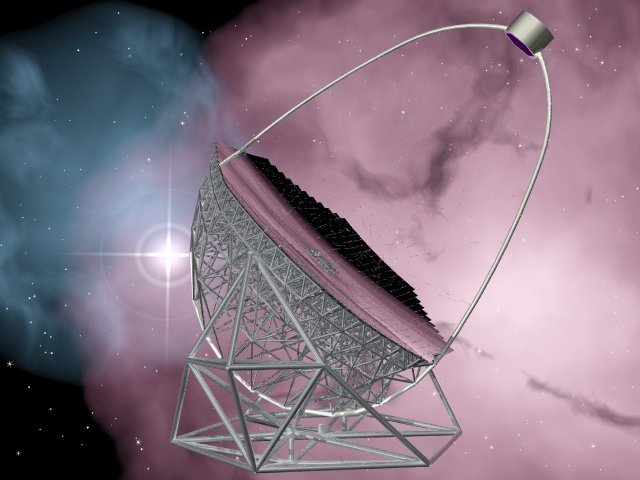
\includegraphics[width=8.5cm]{realmagic1}}
  \vskip 50pt
  {\huge \yo}
  \vskip 50pt
  {\LARGE Septiembre, 2\,000 \\} 
\end{center}

\echapter %%==================================================

\thispagestyle{empty}  

\mbox{} \vskip 20pt

\begin{center}
  {\Huge \sffamily \bfseries \sc \mititulo}
  \vskip 20pt
  
\includegraphics[height=3cm]{escudo_fisicas_0bis}
  \vskip 20pt
  {\large \itshape
    Memoria presentada por  \vskip 25 pt
    {\Large \bfseries \rm \yo}  \vskip 25 pt
    para optar al grado de Doctor en Ciencias F{\'{\i}}sicas. \vskip 40pt
    Dirigida por la profesora \vskip 25pt
    {\Large \bfseries \rm Dra. Mar{\'{\i}}a Victoria Fonseca Gonz{\'{a}}lez}
    } \vskip 35pt
  {\Large \rm Septiembre, 2\,000 \\} \vskip 35pt
  
  {\it \small
    Depto. de F{\'{\i}}sica At{\'{o}}mica, Molecular y Nuclear\\
    Facultad de Ciencias F{\'{\i}}sicas\\
    Universidad Complutense de Madrid\\
    }  
\end{center}

\echapter %%==================================================

\thispagestyle{empty}  

\vspace*{2cm}
\begin{flushright}
  \rule{.7\linewidth}{1pt}\\
  \Large \mititulo
  \rule{.7\linewidth}{1pt}
\end{flushright}
\vspace*{6cm}
\begin{flushright}
  \large 
Jos{\'{e}} Carlos Gonz{\'{a}}lez Garc{\'{\i}}a-Consuegra\\[15 mm]
Depto. F{\'{\i}}sica At{\'{o}}mica, Molecular y Nuclear\\
Facultad de Ciencias F{\'{\i}}sicas\\
Universidad Complutense de Madrid\\[15 mm]
Septiembre, 2\,000
\end{flushright}

\echapter %%==================================================

\thispagestyle{empty}  

\vspace*{2cm} 
%
\hfill 
\parbox[b]{0.65\linewidth}{ 
%
\itshape
%
\raggedright
%
Existe una teor'ia que establece que si alguien alguna vez descubriera
exactamente el por qu'e del Universo y su existencia, 'este
instant'aneamente desaparecer'ia para ser remplazado por algo a'un
m'as ex'otico e inexplicable. \\
%
\vspace{5pt}
\centerline{---}
\vspace{5pt}
%
Existe otra teor'ia que defiende que eso ya ha ocurrido.\\
%
\vspace{15pt}
%
\upshape
%
\raggedleft
%
{\footnotesize (Douglas Adams, ``El restaurante en el fin del Universo'')}
%
} 

\echapter %%==================================================

\endinput
%
%% Local Variables:
%% mode:latex
%% TeX-master: t
%% End:

%%EOF
